\chapter{L' Azienda}
    \section{SogeaSoft S.r.l}
    SogeaSoft S.r.l. è un'azienda di sviluppo \textit{software} fondata nel 1980 a Treviso, con l'obiettivo di progettare e realizzare soluzioni a supporto dei processi aziendali, servendo diverse realtà nel Triveneto.
    Oggi, SogeaSoft rappresenta una filiale di Bluenext S.r.l., azienda di consulenza informatica fondata nel 2012 a Rimini, attiva su tutto il territorio nazionale. Inizialmente, l'azienda acquisitrice si concentrava esclusivamente sullo sviluppo di un \textit{software} per ottimizzare il settore commerciale delle imprese, ma negli ultimi anni ha ampliato il proprio raggio d'azione, esplorando nuovi settori.
    
    \section{Organizzazione aziendale}
    La Figura 1.1 mostra come Sogeasoft S.r.l. sia strutturata in diverse aree operative, ciascuna dedicata alla gestione e allo sviluppo dei prodotti e servizi descritti nei punti seguenti: 
    
    \begin{itemize}
        \item \textbf{SAI}: si occupa dello sviluppo dell'\textit{Enterprise Resource Planning} (ERP), in particolare rappresenta la libreria di base e gestisce la contabilità.
        \item \textbf{SAICon}: sviluppa soluzioni verticali per il settore delle confezioni (abbigliamento) e calzaturiero, integrate con l'ERP SAI.
        \item \textbf{SAIOnWeb}: si concentra su applicativi correlati agli ERP, ma anche su soluzioni autonome come \textit{Customer Relationship Management} (CRM), \textit{Supplier Relationship Management} (SRM), raccolta ordini e \textit{After Sales Service} (ASS). Inoltre, sviluppa la nuova architettura per la migrazione del gestionale.
        \item \textbf{SAIPro}: fornisce applicativi per la pianificazione e il controllo della produzione, destinati alle aziende manifatturiere.
        \item \textbf{BI}: Sviluppa soluzioni per la \textit{Business Intelligence} (BI), focalizzandosi sull'analisi dei dati aziendali per ottimizzare le \textit{performance} e supportare decisioni strategiche più informate e mirate. 
        \item \textbf{CS} (\textit{Customer Service}): offre supporto ai clienti tramite un ufficio dedicato a SAI e un altro dedicato a SAICon, per garantire assistenza mirata.
        \item \textbf{Ufficio sistemistico}: si occupa della gestione dell'infrastruttura \textit{hardware}, sia interna all'azienda che per i clienti che richiedono supporto, oltre a fornire assistenza ai \textit{team} di sviluppo.
    \end{itemize}
    
    \noindent SAIonWeb è stato il tema principale del mio \textit{stage}. Il nome SAIonWeb era inizialmente legato al progetto originale, focalizzato esclusivamente su applicativi utilizzabili tramite il \textit{web}. Tuttavia, con l'evoluzione dell'architettura del sistema, il nome è diventato fuorviante. Attualmente il progetto si occupa di sviluppare un'infrastruttura più moderna e flessibile, che possa eventualmente supportare e gradualmente sostituire il gestionale SAI. 
    Questo processo prevede la collaborazione di membri provenienti da diverse aree, tra cui il \textit{team} di SAICon e quello di SAIPro, che lavorano congiuntamente per integrare i vari componenti del sistema.\\

    \begin{figure}
        \centering
        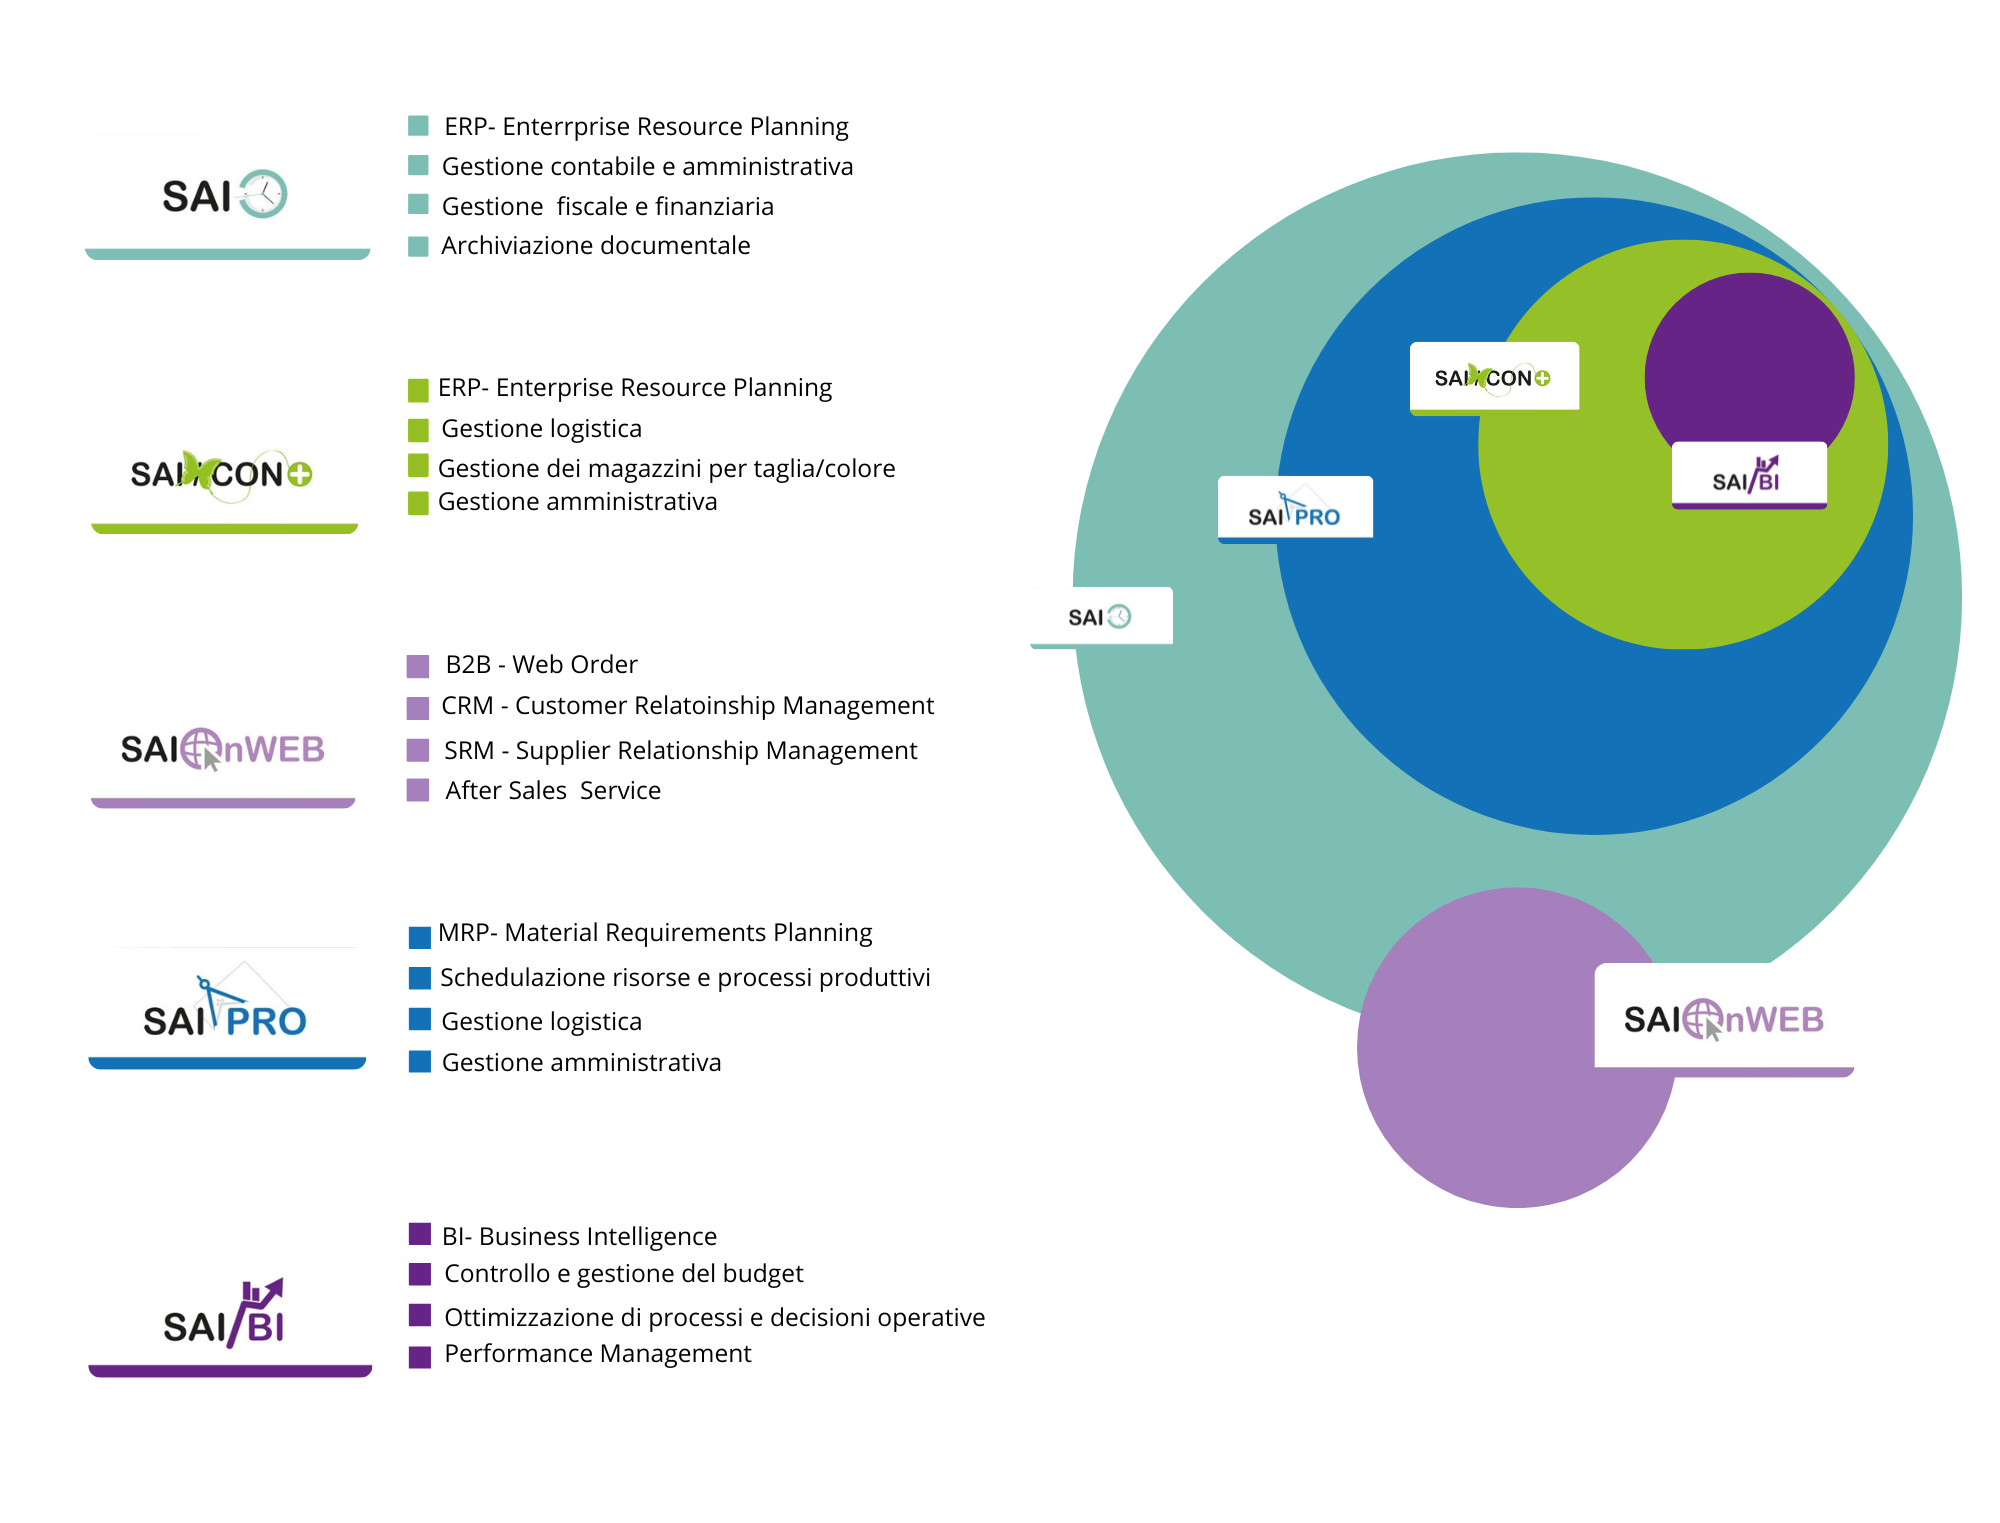
\includegraphics[width=0.9\linewidth]{BCS-Tessi/images/SOGEAProdotti.png}
        \caption{Panoramica dei prodotti e servizi offerti da SogeaSoft}
        \label{fig:panoramica_prodotti}
    \end{figure}

    \noindent Come si può osservare in Figura 1.1, i principali prodotti di SogeaSoft S.r.l. sono strettamente interconnessi, il che si riflette nell’organizzazione dei \textit{team} all’interno dell’azienda. Sebbene esista una divisione indicativa basata sul tipo di prodotto sviluppato, i ruoli risultano essere sfumati e coprono più aree di competenza. 
    \noindent Le persone che lavorano su ciascun prodotto fanno riferimento a un \textit{Product Owner}, che può rappresentare più \textit{team} in base alle necessità.

    \noindent Durante il mio \textit{stage} ho avuto modo di interagire con: 
    \begin{itemize}
        \item \textbf{\textit{Product Owner}}: si occupa di definire la visione del prodotto, gestire il \textit{backlog}, e collaborare con il \textit{team} di sviluppo e gli \textit{stakeholder}.
        \item \textbf{\textit{Team Leader}}: gestisce il \textit{team} di sviluppo. In SogeaSoft S.r.l. questa figura può coincidere con il \textit{Product Owner} e/o con il \textit{Scrum Master}. (non so se tenerlo)
        \item \textbf{Sviluppatore}: si occupa di progettazione, sviluppo e \textit{testing} del \textit{software}. In base al grado di esperienza contribuisce anche all'analisi e all'assistenza ai clienti. 
    \end{itemize}


    \section{Prodotti di SogeaSoft}

    Il prodotto principale di SogeaSoft S.r.l. è un \textit{software} ERP denominato SAI (Sistema Aziendale Integrato). Costituisce la base per tutti gli altri prodotti sviluppati dall'azienda infatti fanno affidamento diretto su SAI. Nasce come software per la gestione della contabilità, poi ampliato con il tempo e adattato a realtà manifatturiere, portando la necessità di introdurre ulteriori funzionalità. 
    Nel contesto del mio stage ho potuto approfondire SAIOnWeb e SAIPro che sviluppano le seguenti funzionalità:
    \begin{itemize}
        \item \textbf{Material Requirements Planning (MRP)}: pianificazione per determinare i materiali necessari per la produzione, ottimizzando i tempi di approvvigionamento e garantendo la disponibilità delle componenti richieste;
        \item \textbf{Master Production Scheduling} (MPS): piano di produzione dettagliato per garantire il rispetto degli impegni con i clienti, ottimizzando l’utilizzo delle risorse e coordinando la produzione con la domanda prevista;
        \item \textbf{Capacity Requirements Planning (CRP)}: analisi delle capacità produttive disponibili per verificare che siano adeguate a soddisfare i requisiti stabiliti dal piano di produzione;
        \item \textbf{Finite Capacity Scheduling (FCS)}: pianificazione dettagliata che considera i limiti effettivi delle risorse aziendali, ottimizzando l'allocazione e la sequenza delle attività produttive per massimizzare l'efficienza.       
    \end{itemize}
    
        \subsection{Target dell'azienda}
        SogeaSoft S.r.l. si rivolge principalmente alle Piccole e Medie Imprese (PMI), che spesso presentano la necessità di digitalizzare i propri processi aziendali, richiedendo al contempo un supporto tecnico affidabile e costante.  
        
        \noindent Le PMI che rappresentano il target principale dell’azienda operano prevalentemente nel settore manifatturiero e sono interessate a ottimizzare i propri flussi operativi. Questi includono la gestione e il monitoraggio delle \textit{performance} del personale, la regolazione e l’automazione dei processi logistici, e l’implementazione di soluzioni che migliorino la pianificazione, la produzione e il controllo dei costi.
        
    \section{Modello di sviluppo}
    SogeaSoft S.r.l. ha adottato un modello di sviluppo software basato sul \textit{framework} Scrum, una metodologia ispirata ai principi dell’Agile Manifesto. Questo approccio mira a ottimizzare il processo di lavoro rendendolo modulare, adattivo e in grado di rispondere rapidamente ai cambiamenti e alle necessità del cliente e alla complessità delle commesse.  
    
    \noindent Alla base di Scrum vi è il concetto di \textit{User Story}, una descrizione ad alto livello delle funzionalità attese dal cliente o individuate dal \textit{Product Owner}. Le \textit{User Story}, raccolte nel \textit{Product Backlog}, costituiscono l'insieme di attività prioritarie che guidano lo sviluppo. Questo elenco viene costantemente aggiornato per riflettere nuove necessità o modificare le priorità.
    
    \noindent Dopo essere state definite e raffinate, le \textit{User Story} guidano l'organizzazione e la pianificazione dello sviluppo, che avviene attraverso cicli iterativi chiamati \textit{Sprint}. Questo approccio consente di garantire un miglior controllo dei processi e un allineamento costante tra il \textit{team} di sviluppo e gli obiettivi aziendali. 

    \noindent Le principali cerimonie Scrum adottate sono visibili in un diagramma nella Figura 1.2, meglio descritte in seguito:
    \begin{itemize}
    
        \item \textbf{\textit{Sprint Planning}}: all'inizio di ogni \textit{Sprint}, il gruppo di lavoro partecipa a una sessione di pianificazione per selezionare gli elementi del \textit{backlog} da sviluppare. Gli obiettivi principali dello \textit{Sprint} vengono definiti insieme allo \textit{Sprint Goal}, che rappresenta il risultato principale atteso. Le attività vengono poi suddivise in compiti più piccoli, stimati tramite la sequenza di Fibonacci, per garantire una gestione efficace delle tempistiche;

        \item \textbf{\textit{Daily Scrum}}: ogni giorno, il gruppo di sviluppo e lo \textit{Scrum Master} partecipano a un incontro breve, durante il quale si coordinano le attività e si identificano eventuali ostacoli. Questo garantisce un allineamento costante del gruppo verso gli obiettivi dello \textit{Sprint};

        \item \textbf{\textit{Sprint Review}}: alla fine dello \textit{Sprint}, gli incrementi di prodotto sviluppati vengono presentati. Sebbene in teoria questa fase preveda il coinvolgimento degli \textit{stakeholder}, nel caso di SogeaSoft S.r.l. il ruolo di collegamento con il cliente finale viene svolto dal \textit{Product Owner}, il quale raccoglie \textit{feedback} e li traduce in aggiornamenti per il \textit{backlog};  

        \item \textbf{\textit{Sprint Retrospective}}: questo momento di riflessione sul lavoro svolto è utilizzato dal gruppo di lavoro per identificare opportunità di miglioramento nel processo di sviluppo. Tuttavia, data la dimensione contenuta dei \textit{team} e la consolidata organizzazione del lavoro, questa cerimonia viene svolta solo quando necessario.  

        \item \textbf{Raffinamento del \textit{Backlog}}: un'altra attività fondamentale è quella del Raffinamento, che si tiene con cadenza regolare per preparare gli elementi del \textit{backlog} per i successivi \textit{Sprint}. Durante queste sessioni, il gruppo di lavoro collabora per suddividere le funzionalità più complesse in elementi più piccoli, chiarire i requisiti e definire criteri di accettazione. Questo processo garantisce che gli elementi siano chiari e pronti per essere inclusi nel prossimo \textit{Sprint Planning}. La responsabilità principale di questa attività ricade sul \textit{Product Owner}, con il supporto del \textit{team} di sviluppo.
        
    \end{itemize}
    
    \noindent In sintesi, il modello di sviluppo di SogeaSoft si basa su una gestione iterativa e collaborativa, che consente di rispondere in modo agile alle richieste dei clienti e di mantenere un flusso di lavoro efficace e focalizzato sugli obiettivi aziendali.

    \begin{figure}[H]
        \centering
        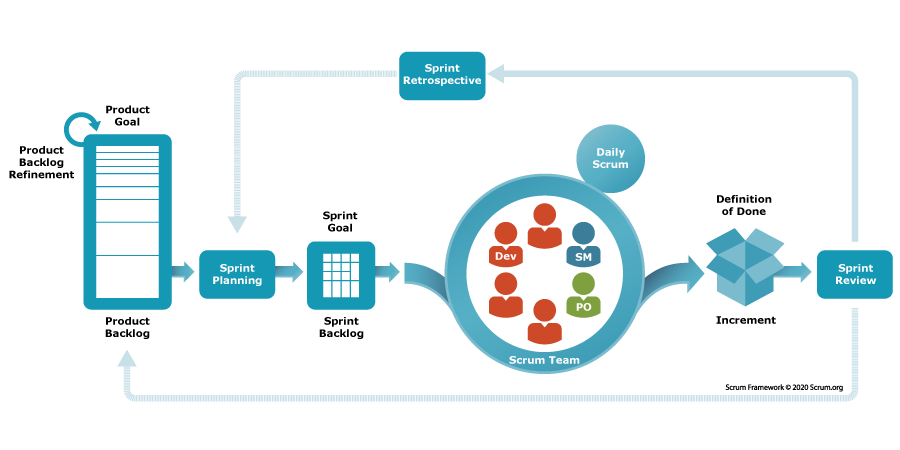
\includegraphics[width=0.8\linewidth]{BCS-Tessi/images/scrum_flow.png}
        \caption{Diagramma del flusso di lavoro del modello Scrum, basato sulla filosofia Agile}
        \label{fig:scrum_flow}
    \end{figure}
    
    \section{Organizzazione interna}
    SogeaSoft S.r.l. implementa i principi della norma \textbf{UNI EN ISO 9001:2015} per garantire un sistema di gestione della qualità dei prodotti efficace.
    
    \noindent Pur non essendo specificamente pensata per lo sviluppo \textit{software}, la norma trova applicazione nell’organizzazione grazie all’adozione di pratiche volte a standardizzare i processi e migliorare l’efficienza operativa. L'azienda basa la propria struttura sull'approccio per processi, suddividendo il lavoro in unità specializzate (come SAI, SAIPro e SAICon) e adottando metodologie \textit{Agile} per la pianificazione e gestione delle attività, ispirandosi allo standard ISO/IEC/IEEE 12207 (\textit{Systems and software engineering - Software life cycle processes}).

    \noindent Anche i principi dell’approccio per processi e del metodo Plan-Do-Check-Act (PDCA) sono applicati in tutte le fasi operative. Il PDCA si concretizza attraverso la pianificazione accurata delle attività (Plan), la loro esecuzione (Do), l’analisi dei risultati ottenuti (Check) e l’implementazione di eventuali azioni correttive o migliorative (Act).

    \noindent Un esempio evidente dell’applicazione del PDCA è riscontrabile nel modello di sviluppo Scrum, adottato da SogeaSoft S.r.l.per garantire iterazioni rapide e flessibili. Durante gli \textit{Sprint}, il \textit{backlog} viene pianificato e raffinato (\textit{Plan}), le attività vengono eseguite secondo le priorità stabilite (\textit{Do}), e i risultati sono presentati e analizzati attraverso la \textit{Sprint Review} e la \textit{Retrospective} (\textit{Check}). Eventuali miglioramenti vengono quindi incorporati negli \textit{Sprint} successivi (\textit{Act}).
    
    \noindent La Figura 1.3 mostra il certificato UNI EN ISO 9001:2015 ottenuto dall’azienda, che conferma l’impegno di SogeaSoft S.r.l. nel mantenere elevati standard di qualità nei propri processi.

    \begin{figure}[H]
        \centering
        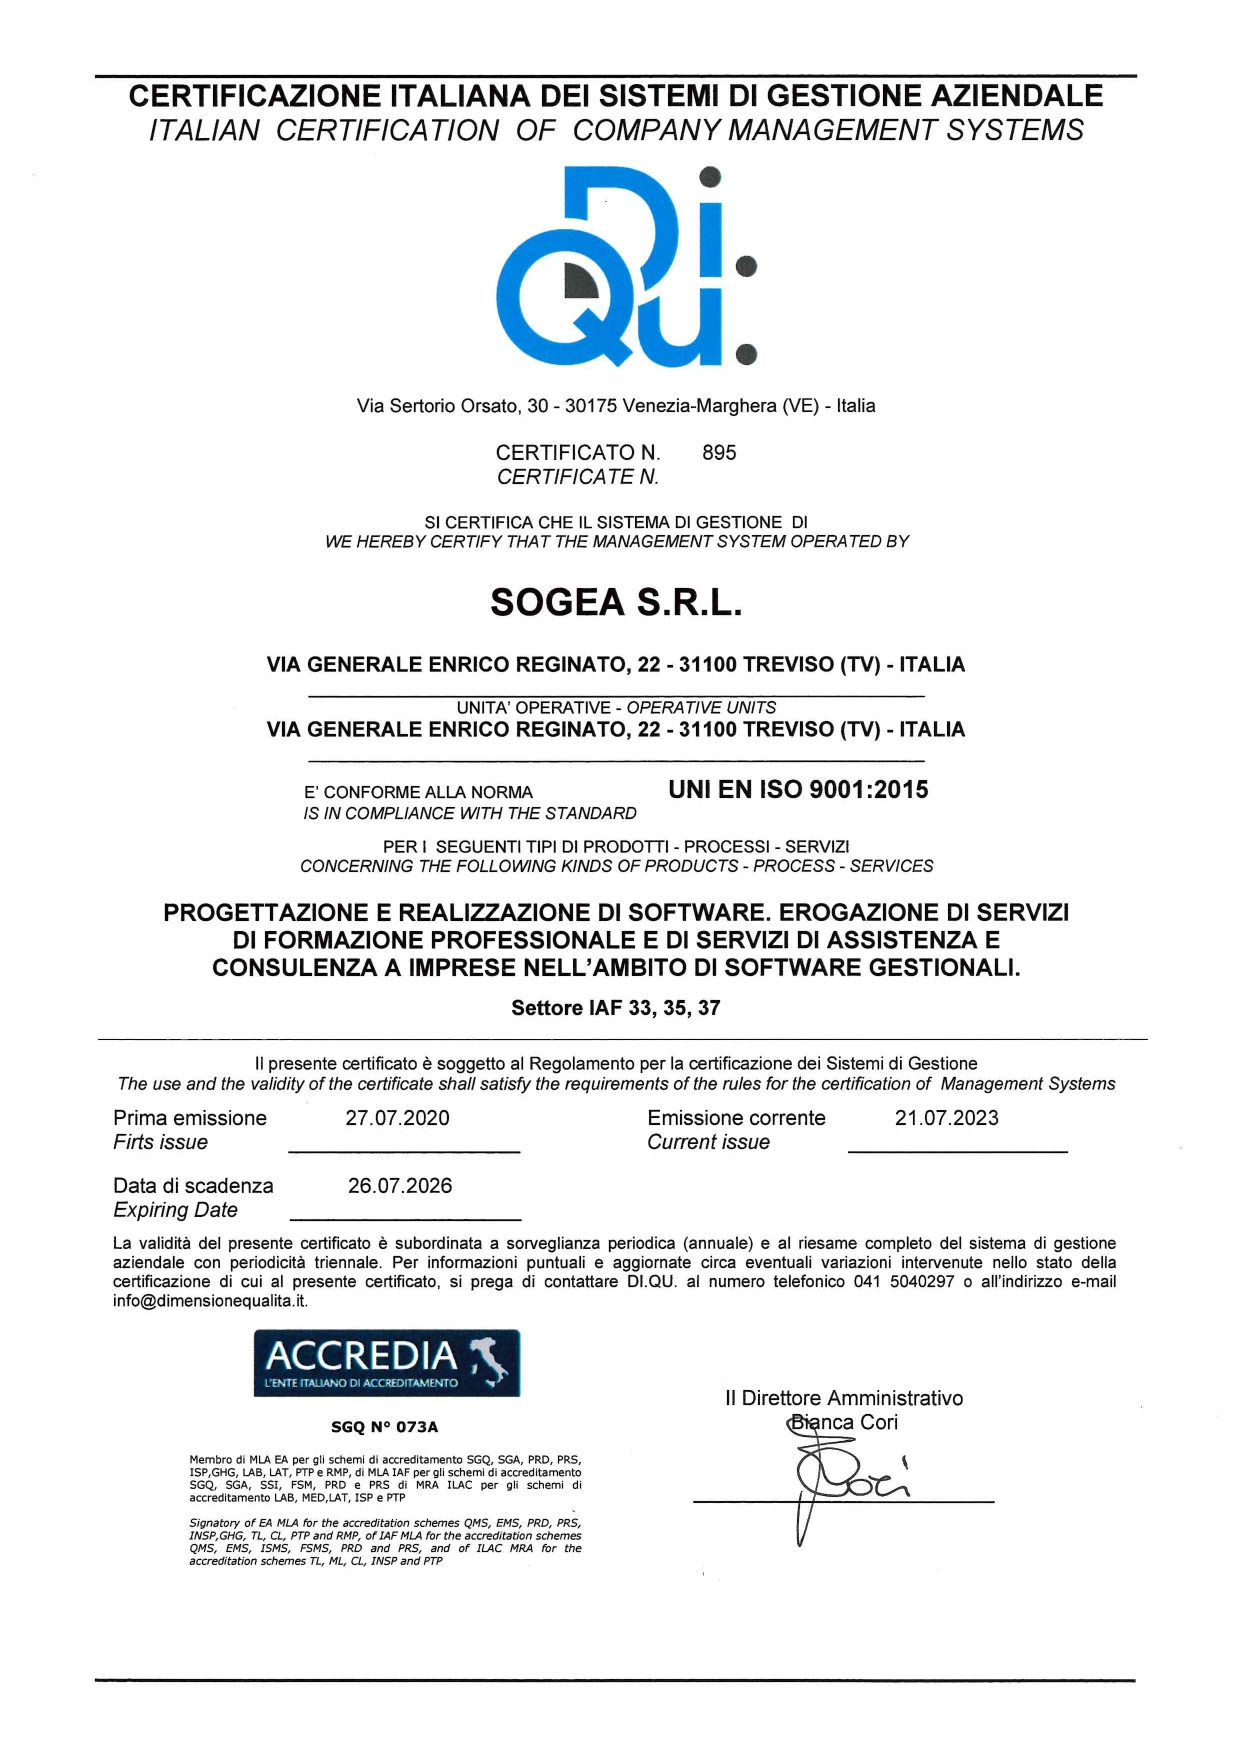
\includegraphics[width=0.5\linewidth]{BCS-Tessi/images/CertificatoSogea.jpg}
        \caption{Figura 1.3: Certificazione ISO ottenuta da SogeaSoft S.r.l.
        Fonte: https://sogeasoft.com/p/iso9001 \textit{(ultimo accesso 26/02/2025)}}
        \label{fig:certificazione-iso}
    \end{figure}

    \noindent Nelle successive sezioni approfondirò i processi di ciclo di vita del \textit{software} a cui ho avuto modo di partecipare durante il mio \textit{stage}. In particolare, riferendomi allo standard ISO/IEC/IEEE 12207:2017 tratterò i seguenti capitoli: Processi organizzativi e abilitanti e Processi di Gestione Tecnica.
    
    
        \subsection{Gestione della configurazione}
        Lo scopo del processo di Gestione della configurazione è stabilire e mantenere l'integrità di tutti gli \textit{output} identificati di un progetto o processo e renderli disponibili alle parti interessate. (ref: iso/iec)\\
        \noindent Nello specifico, un sistema di controllo è importante nell'evoluzione delle funzionalità del software, del codice e della documentazione associata perché essi costituiscono gli \textit{output} in questione. Ciò permette di mantenere traccia delle modifiche e garantire che ogni versione sia controllata, riproducibile e coerente con i requisiti stabiliti, facilitando così la gestione delle evoluzioni del \textit{software} e la collaborazione tra i membri del \textit{team}. 

        \noindent In SogeaSoft S.r.l. il controllo delle modifiche al codice avviene attraverso un \textit{Version Control System} (VCS), che traccia l’evoluzione del \textit{software} in modo strutturato. Le versioni del codice vengono archiviate all’interno di \textit{repository}, strutture dati appositamente organizzate per gestire i cambiamenti. 
        \noindent Queste \textit{repository} si basano su tre principali tipologie di \textit{branch}:  
        \begin{itemize}
            \item \textbf{master}: rappresenta la versione stabile destinata alla produzione, aggiornata manualmente in concomitanza con ogni rilascio ufficiale e avanzamento di versione; 
            \item \textbf{develop}: funge da \textit{branch} principale per lo sviluppo, raccogliendo le nuove funzionalità prima della loro distribuzione al Cliente; 
            \item \textbf{release}: include i \textit{branch} dedicati ai rilasci personalizzati, specifici per ogni cliente.  
        \end{itemize}

        \noindent La documentazione viene gestita all'interno di un'area dedicata dell'ambiente di sviluppo adottato (Sezione 1.5.2) da SogeaSoft S.r.l., denominata Wiki. Questo sistema organizza le informazioni in base ad argomenti, capitoli e finalità d'uso, garantendo una struttura relativamente chiara. Inoltre, ogni modifica è accompagnata da un \textit{timestamp} e dall'identificativo dell'autore, permettendo un tracciamento preciso delle revisioni. 
        
        \subsection{Gestione dell’informazione}

        Lo scopo del Processo di Gestione delle Informazioni è garantire alle parti designate l’accesso a informazioni pertinenti, tempestive, complete e valide durante e, ove opportuno, dopo il ciclo di vita del sistema (ref. ISO/IEC, par. 6.3.6).  

        \noindent Sogea S.r.l. impiega la piattaforma Microsoft Azure sia per la scrittura del codice sia per la gestione della documentazione aziendale. Questo strumento collaborativo facilita l'integrazione con diversi sistemi di supporto ai processi di Gestione della Configurazione, Progettazione, Implementazione e Manutenzione. In particolare, per la documentazione, SogeaSoft S.r.l. utilizza le Wiki, che consentono di organizzare e strutturare le informazioni in modo sistematico.  

        \begin{figure}[H]
            \centering
            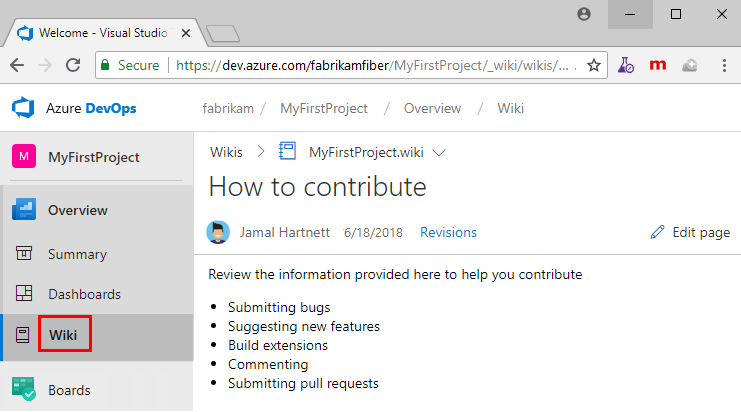
\includegraphics[width=0.5\linewidth]{BCS-Tessi/images/wiki_microsoft.png}
            \caption{Figura 1.4: Esempio di Wiki in Azure. Fonte: https://learn.microsoft.com/it-it/azure/devops/project/wiki/wiki-create-repo?view=azure-devopstabs=browser \textit{(ultimo accesso 1/03/2025)}}
            \label{fig:Wiki}
        \end{figure}

        \noindent Durante il mio \textit{stage}, ho osservato come, data l’interoperabilità del \textit{software} aziendale, risulti fondamentale che la documentazione associata sia formalmente strutturata in documenti accessibili a tutti i membri dei \textit{team}. Tale documentazione segue una gerarchia ben definita, comprendente la registrazione di incontri, requisiti, analisi e scelte progettuali, tutte adeguatamente descritte e motivate.  

        \noindent Tuttavia, questo approccio non è sempre stato adottato in maniera sistematica. Nelle versioni più datate del \textit{software}, la documentazione risultava spesso incompleta o assente, costringendo gli sviluppatori a ricorrere al \textit{reverse engineering} per comprendere il funzionamento del codice. Questa criticità ha generato una forte dipendenza dalle conoscenze dei singoli sviluppatori coinvolti nel processo iniziale, rendendo più complesso l’apporto di modifiche e aggiornamenti successivi.  

        \noindent Da qui deriva la necessità di SogeaSoft S.r.l. di abbandonare gradualmente il vecchio sistema in favore di un nuovo sistema più documentato, decentralizzato e flessibile. 
        
        \subsection{Processi di formazione}

        Durante il mio stage ho avuto modo di analizzare le modalità adottate da SogeaSoft S.r.l. per la formazione dei propri dipendenti. L'azienda implementa un approccio articolato, combinando diverse metodologie formative per garantire un apprendimento efficace e continuo. In particolare, le strategie impiegate comprendono:

        \begin{enumerate}
        \item \textbf{Lezioni in presenza}: nel caso in cui l’azienda intenda introdurre nuove tecnologie o apportare modifiche significative ai \textit{software} in uso, vengono organizzati corsi di formazione condotti da esperti del settore.

        \item \textbf{Autoapprendimento}: successivamente alle lezioni frontali, i dipendenti sono incoraggiati a integrare e approfondire autonomamente le conoscenze acquisite. Tale processo avviene attraverso la consultazione di libri tecnici, la visione di videolezioni su piattaforme online gratuite e l’analisi di progetti preesistenti affini.

        \item \textbf{Peer programming}: questa pratica collaborativa prevede il coinvolgimento di due o più programmatori nella scrittura del codice, promuovendo la condivisione di competenze e il miglioramento della qualità del \textit{software}. Solitamente, essa si concretizza nell’affiancamento di un programmatore esperto a uno meno esperto, con l’obiettivo di favorire un apprendimento diretto e pratico secondo il principio del \textit{learn by doing}.
        \end{enumerate}
        
        \noindent Nel corso del mio stage ho applicato prevalentemente le metodologie di \textbf{autoapprendimento} e \textit{\textbf{peer programming}}. Come si può osservare in Figura 1.5, nelle prime settimane la ricerca autonoma di informazioni e il confronto diretto con colleghi più esperti hanno occupato gran parte della mia giornata lavorativa. Tuttavia, con il progressivo consolidamento delle competenze acquisite, dopo circa dieci giorni lavorativi ho potuto ridurre significativamente il tempo dedicato allo studio individuale, limitando il ricorso al \textit{peer programming} ai soli casi in cui si presentassero difficoltà specifiche nello sviluppo del \textit{software}.

        \begin{figure} [H]
            \centering
            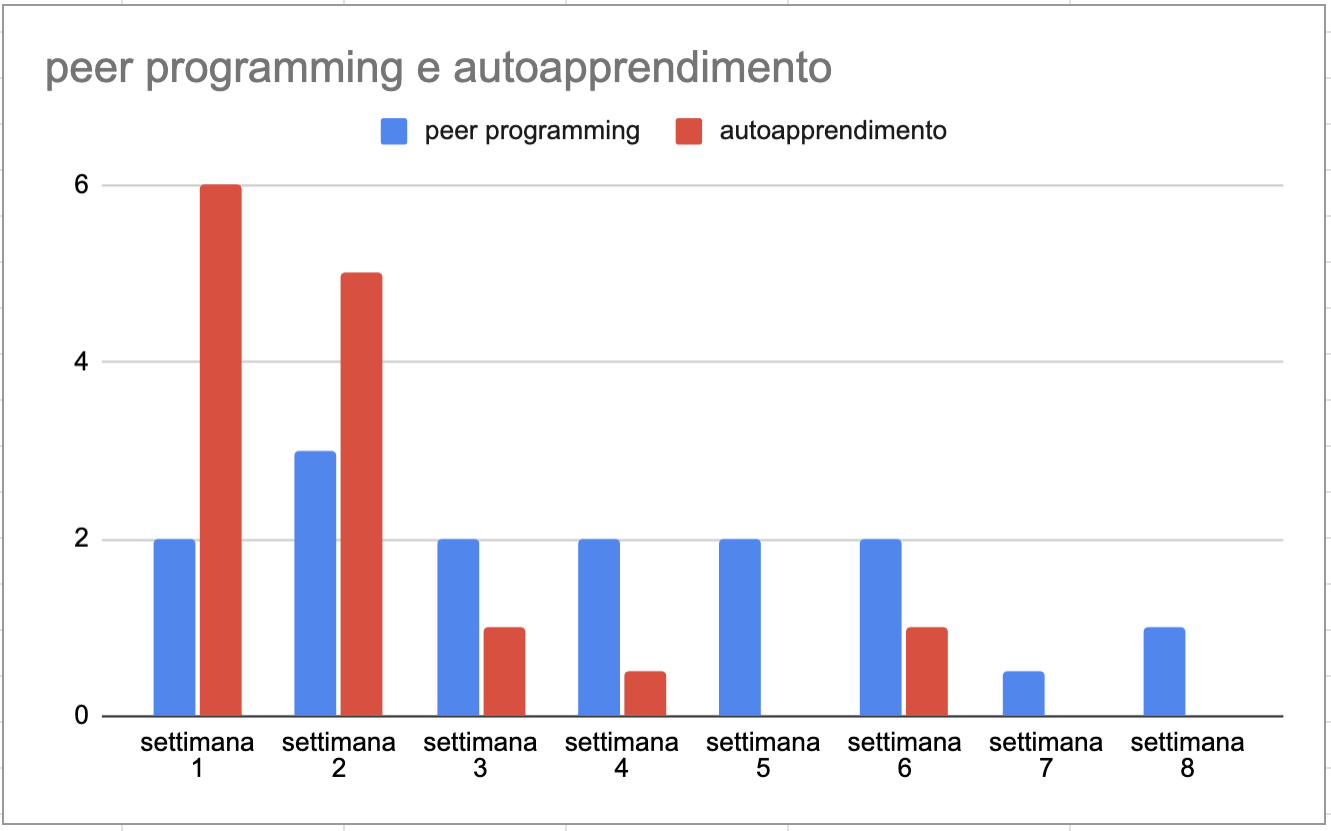
\includegraphics[width=0.8\linewidth]{BCS-Tessi/images/Ore_formazione.png}
            \caption{Rendicontazione ore dedicate ai processi di formazione durante il mio stage}
            \label{fig:Ore-formazione}
        \end{figure}
        

    \section{Ciclo di vita di un progetto software}
    Scriverò una breve introduzione al ciclo di vita di un progetto software: che cos’è e in cosa
    consistono le sue fasi, approfondite nelle seguenti sezioni.
        \subsection{Analisi preliminare e raccolta dei requisiti}
        Scriverò una descrizione dettagliata dell’attività di analisi dei bisogni degli stakeholder e di
        raccolta dei requisiti che il progetto software dovrà soddisfare.
        \subsection{Progettazione}
        Scriverò una descrizione del processo di progettazione: in cosa consiste, come viene attuato
        dall’azienda, quali risultati produce.
        \subsection{Sviluppo}
        Scriverò una descrizione dell’attività di implementazione delle soluzioni individuate nella
        fase precedente e tutte le attività a supporto di essa.
        \subsection{Verifica e Validazione}
        Scriverò una descrizione delle attività di verifica del codice per garantire la conformità ai
        requisiti definiti e l'assenza di errori. Descrizione dettagliata delle varie tipologie di test a       pplicate.
        Aggiungerò una descrizione delle attività finalizzate a garantire che il prodotto software
        soddisfi i requisiti del cliente e risponda correttamente alle sue      esigenze operative
        (validazione).
        \subsection{Manutenzione}
        Scriverò una descrizione dei processi finalizzati alla manutenzione regolare del prodotto per
        garantire il soddisfacimento di bisogni e di requisiti che variano con il tempo.
    \section{Tecnologie utilizzate}
    Scriverò una descrizione dettagliata di tutte le tecnologie utilizzate dall’azienda specificamente nello
    sviluppo software. Ai fini di questa trattazione descriverò anche le tecnologie obsolete che non sono
    più utilizzate dai dipendenti ma che sono ancora in uso nei meandri del prodotto principale
    dell’azienda SogeaSoft S.r.l.
    Nello specifico descriverò: linguaggi di programmazione, tecnologie alla base dei prodotti
    d   ell’azienda, l’ambiente di sviluppo, gli editor utilizzati, e       strumenti per i processi di verifica.
    \section{L’innovazione in Sogea}
    Scriverò una descrizione accurata della propensione all’innovazione di Sogea, spiegando le concrete
    misure che l’azienda sta adottando a tal proposito. Includerò come Bluenext abbia contribuito in ciò.